\documentclass[11pt,letterpaper]{report}
\usepackage[margin=0.75in]{geometry}
\usepackage[latin1]{inputenc}
\usepackage{amsmath}
\usepackage{amsfonts}
\usepackage{amssymb}
\usepackage{graphicx}
\usepackage{color}
\graphicspath{{./images/}{IR}}
\usepackage{fancyhdr}
\pagestyle{fancy}
\fancyhead{}
\lhead{CS333}
\chead{Project 2 Report}
\rhead{Andy Keene}
\author{Andy Keene}
\title{Project Two Report\\Introduction to Operating Systems\\ Spring 2017}
\date{}
\begin{document}
	\maketitle
	

	\section*{Description}
	For this assignment, I learned about locks used for concurrent data structures in the kernel; expanded the process structure to contain ownership information and CPU use-time; implemented new user commands to see current process statuses, and track the run-time of user level commands; and how to use wrappers for system calls that effect files or access the proc table data structure . \\
		
	\section*{Deliverables}
	The following features were added to xv6:
	
	\begin{itemize}
	
	\item New system calls to support process ownership and retrieve active process information
	 	\begin{itemize}
			\item setuid sets the UID of the current process to \emph{value} 
				\begin{verbatim}
					int
					setuid(uint value);
				\end{verbatim}
				
			\item setgid sets the GID of the current processes to \emph{value} 
				\begin{verbatim}
					int
					setgid(uint value);
				\end{verbatim}
				
			\item getuid returns the UID of the current process
				\begin{verbatim}
					int
					getuid(void);
				\end{verbatim}
			
			\item getgid returns the current GID of the current process
				\begin{verbatim}
					int
					getgid(void);
				\end{verbatim}
			
			\item getppid returns the PPID (parent process ID) of the current process
				\begin{verbatim}
					int
					getppid(void);
				\end{verbatim}
				
			\item getprocs fills in the provided {\tt uproc} structure with information of the currently active processes
			         up to a maximum number of the given {\tt max} and returns the number of processes placed in the table.
			         \begin{verbatim}
					int
					getprocs(uint max, struct uproc *table);
				\end{verbatim}         

		 \end{itemize}
	
	\item Process total CPU time. Each process now stores {\tt cpu\_ticks\_in} (the most recent time it started running) and {\tt cpu\_ticks\_total} 
		(the total time spent in the CPU) so that the process's total time running can be tracked and calculated.
	
	\item A new user command, {\tt ps}, that prints the current statues of active processes to the standard output.
	
	\item A new user command,  {\tt time}, that will time the execution of commands.
	
	\item A modification of the {\tt ctrl-p} console command to include the {\tt uid}, {\tt gid}, {\tt ppid}, and total execution time information of each 
		currently running process. 
		
	\end{itemize}
	
\newpage	
	\section*{Implementation}
	
	
	\subsection*{New System Calls For Process}
	Using the process outlined in project one, the following system calls were implemented by adding: a user-side header in {\tt user.h}; 
	creating a system call number in {\tt syscall.h}; updating the system call jump table, the system call name table, and adding a kernel side
	header in {\tt syscall.c}; 
	a user-side stub in {\tt usys.S}; and implementation in {\tt sysproc.c}. To support process ownership new fields {\tt uint uid} and {\tt uint gid}
	were added to the {\tt proc} structure definition in proc.h (lines 61-62). INITUID and INITGID
	were defined in param.h (lines 15-16) with which to initialize these fields for the {\tt init} process in proc.c (lines 108-109). All other processes
	inherit their UID, GID from their parent process in fork (proc.c lines 169-170). Since the process stores a pointer to its parent, any PPIDs will be 
	calculated on the fly. Each new system call's description and it's corresponding file changes are as follows:

		\begin{itemize}

			\item The {\tt setuid()} system call sets the process's UID to the given \emph{value}. This \emph{value} is retrieved from the stack
				as an {\tt int} using {\tt argint()} before being cast to an {\tt uint}, where $0 \leq value \leq 32767$. If {\tt setuid()} fails to 
				retrieve the argument from the stack or if the given \emph{value} is out of bounds then $-1$ is returned while
				 upon success $0$ is returned. The files modified to support
				this system call are as follows:
				
					\begin{itemize}
					
					\item user.h (line 35)
					\item usys.S (line 37)
					\item syscall.h (line 29)
					\item syscall.c (lines 106, 138, 172)
					\item sysproc.c (lines 129-142)
					
					\end{itemize}
			
				The function prototype is:
				\begin{verbatim}
					int
					setuid(uint value);
				\end{verbatim}
				
			\item The {\tt setgid()} system call sets the process's GID to the given \emph{value}. This \emph{value} is retrieved from the stack
				as an {\tt int} using {\tt argint()} before being cast to an {\tt uint}, where $0 \leq value \leq 32767$ (it was passed from the user side as a {\tt uint} so this
				conversion is safe). If {\tt setgid()} fails to 
				retrieve the argument from the stack or if the given \emph{value} is out of bounds then $-1$ is returned while upon success $0$ is 				
				returned. The files modified to support
				this system call are as follows:
				
					\begin{itemize}
					
					\item user.h (line 36)
					\item usys.S (line 38)
					\item syscall.h (line 30)
					\item syscall.c (lines 107, 139, 173)  
					\item sysproc.c (lines 144-157)
					
					\end{itemize}
					
					The function prototype is:
					\begin{verbatim}
						int
						setgid(uint value);
					\end{verbatim}
				
			\item The {\tt getuid()} system call returns the process's UID. This system call cannot fail and will simply return whatever value is stored as UID
				 in the calling process as a {\tt uint}. If this value is out of bounds it would imply that the {\tt setuid()} system call or the defined initial values are incorrect. 
				 The files modified to support this system call are as follows:
				 
					 \begin{itemize}
					
					\item user.h (line 32)
					\item usys.S (line 34)
					\item syscall.h (line 26)
					\item syscall.c (lines103, 135, 169)
					\item sysproc.c (lines 110-114)
					
					\end{itemize}
					
					The function prototype is:
					\begin{verbatim}
						uint
						getuid(void);
					\end{verbatim}
			
			\item The {\tt getgid()} system call returns the process's GID. This system call cannot fail and will simply return whatever value is stored in the GID
				field of the calling process as a {\tt uint}. The files modified to support this system call are as follows:
				 
					 \begin{itemize}
					
					\item user.h (line 33)
					\item usys.S (line 35)
					\item syscall.h (line 27)
					\item syscall.c (lines 104, 136, 170)
					\item sysproc.c (lines 116-120)
					
					\end{itemize}
					
					The function prototype is:
					\begin{verbatim}
						uint
						getgid(void);
					\end{verbatim}
			
			\item The {\tt getppid()} system call returns the process's PID (parent ID). This system call also cannot fail and will simply return the {\tt pid} field of the parent 				
			process as a {\tt uint}. Note that the initial process, {\tt init}, is considered it's own parent (special case). 
			 	The files modified to support this system call are as follows:
				 
					 \begin{itemize}
					
					\item user.h (line 34)
					\item usys.S (line 36)
					\item syscall.h (line 28)
					\item syscall.c (lines 105, 137, 171 )
					\item sysproc.c (lines 122-127)
					
					\end{itemize}
					
					The function prototype is:
					\begin{verbatim}
						uint
						getppid(void);
					\end{verbatim}
				
			\item The {\tt getprocs()} system call fills in the {\tt uproc} table array given as a parameter for \emph{at most} the given {\tt max} number of
				processes. The user, or calling process, is responsible for correctly allocating an array of {\tt uproc} structures and passing in a valid maximum value (i.e. a 
				valid index). {\tt getprocs()} uses the helper functions {\tt getptr()} to retrieve the pointer to the {\tt uproc} table from the stack, and 
				{\tt getint()} to retrieve the {\tt max} argument. If {\tt getprocs} fails to retrieve the arguments from the stack then $-1$ is returned where a 
				return value greater than or equal to $0$ indicates how many individual process statuses were placed in the table. Additionally since 
				{\tt getprocs} must access the {\tt ptable} data structure, the system call {\tt getprocs()} in sysproc.c acts as a wrapper for the {\tt getprocs} 
				function defined in proc.c. 
		
					The files modified to support this system call are as follows:
				 
					 \begin{itemize}
					
					\item user.h added the struct uproc type declaration (line 3), and the system call function header (line 37)
					\item usys.S (line 39)
					\item syscall.h (line 31)
					\item syscall.c (lines 108, 140, 174)
					\item sysproc.c  defines the wrapper system call function (lines 159-172) which must include {\tt uproc.h}
						(line 9) to use the given {\tt  uproc} pointer.
					\item proc.c defines the core function of the {\tt getproc()} system call (lines 559-591). Here the {\tt ptable} is accessed, using
						the given spin lock, and the {\tt states} array is used to define the string corresponding to process state; 
						 process information is copied into the {\tt uproc} table accordingly. 
					\item uproc.h file was added and defines the {\tt uproc struct} which is also outlined below
					\item defs.h added the {\tt uproc} type declaration (line 11) and {\tt getprocs} function prototype (line 122)  implemented in proc.c 
						so that it may be called from sysproc.c.
					
					\end{itemize}

					The function prototype is:
			       		 \begin{verbatim}
					int
					getprocs(uint max, struct uproc *table);
					\end{verbatim}
					
					The uproc structure (with {\tt STRMAX} defined as 32) is:
					\begin{verbatim}
					struct uproc {
					    uint pid;
					    uint uid;
					    uint gid;
					    uint ppid;
					    uint elapsed_ticks;
 					  uint cpu_total_ticks;
					    uint size;
					    char state[STRMAX];
					    char name[STRMAX];
					};
					\end{verbatim}
					
		\end{itemize} 
	
	\subsection*{Process Execution Time}
	The following files were modified to support tracking the execution time of a process:
	
		\begin{itemize}
			\item {\tt cpu\_ticks\_total} and {\tt cpu\_ticks\_total} were added to the {\tt proc} structure defined in proc.h (lines 72-73)
				to track the most recent time the process was scheduled to run in the CPU, and to count the total time running on the CPU respectively. 
				
			\item These fields are updated, before and after the process runs, in the scheduler and de-scheduler routines in proc.c (lines 320, 363). 
				Each field is set to $0$ during {\tt allocproc} (lines 70-71).

		\end{itemize}
	
	\subsection*{New User Commands}
	
	\begin{itemize}
			\item The new user command {\tt time} was added to calculate and display the time elapsed to run the command that follows it. For example
				{\tt time echo "abc"} will allow {\tt echo} to execute and then display the time it took to do so. The file time.c was added and contains the
				program to run this user command. The {\tt time} user command was also added to the Makefile (line 158).
				
			\item The new user command {\tt ps} was added to display currently active process information to standard-out using the new {\tt getprocs()} system call.
				It is written to display up to a maximum of 64 processes. 
				The file ps.c was added and contains the program to run for this user command. The {\tt ps} user command was also added to the Makefile (line 157).
			
			\item Additionally a new user command {\tt test} was added to help automate testing for the new system calls pertaining to UID, GID, and PPID. The program, 
				found in the new test.c file, demonstrates adding valid and invalid UIDs and GIDs as well as testing \emph{if} GIDs and UIDs are correctly inherted from
				the parent process.  The {\tt ps} user command was also added to the Makefile (line 156).

		\end{itemize}
				
	\subsection*{ctrl-p Modifications}
	The ctrl-p console command prints debugging information to the console. 	{\tt procdump} was refactored in proc.c to print process information in a prettier fashion using a
	helper function {\tt printnum} (lines 515-522) -- and to include the process UID, GID, PPID, and CPU run-time in its output (lines 538, 546-549). Since {\tt elapsed\_time} was 
	implemented in project 1, and {\tt cpu\_total\_ticks} is already calculated no additional calculation were needed. 	




	\newpage
	
	
	
	\section*{Testing}
	
	\subsection*{Valid set UID/GID}
	To test that the {\tt setuid()} and {\tt setgid()} system calls correctly set \emph{valid} numbers we will use the user command {\tt test} to help automate the process of 
	1) Pause to press ctrl-p and see the current UID/GID of the {\tt test} process
	2) Print the number's $x$, where $x$ is in the valid range for the UID and GID fields (11 and 50 will be used)
	3) Call {\tt setuid()}/{\tt setgid()} with $x$ 
	4) Pause before exiting to allow the user to press {\tt ctrl-p} and see what number the UID/GID is set to for {\tt test} user process in the ptable and 
	4) print the return code of the system call. 
	For both {\tt setuid()} and {\tt setgid()} both a return code of $0$ and an output of {\tt ctrl-p} displaying the number $x$ for the respective UID/GID field is expected.

\begin{figure}[h!]
\centering
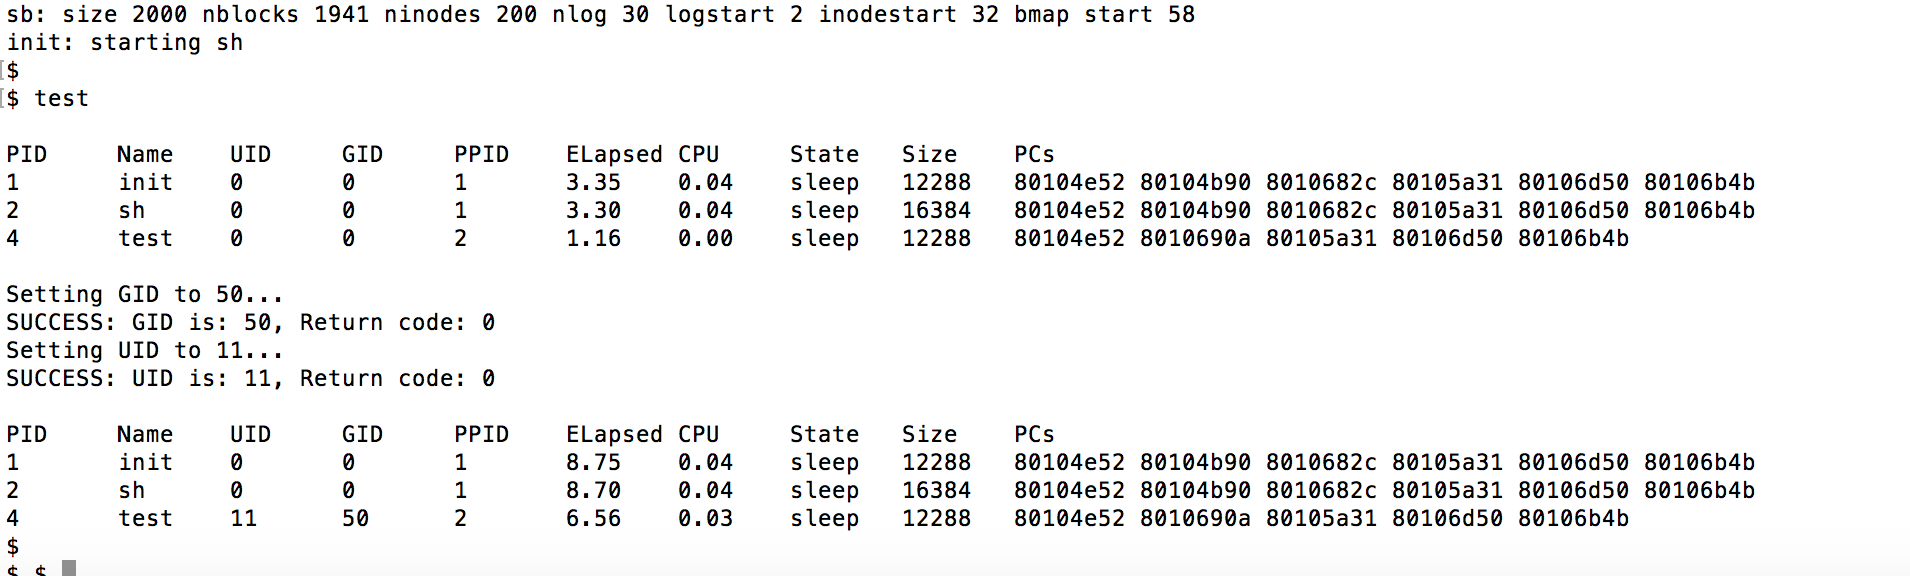
\includegraphics[width=0.8\linewidth]{setuid-setgid.png}
\caption[valid setuid() and setgid()]{valid setuid() and setgid()}
\label{fig:datetest}
\end{figure}	
	
	Because the initial UID/GID shown by ctrl-p were shown as 0, {\tt setgid()} was called with 50, {\tt setuid()} was called with 11, and ctrl-p shows a GID of 50 and UID of 11 for test immediately after with return codes of $0$ (success) for each call, this test \textbf{PASSES}.


	\subsection*{Invalid set UID/GID}
	To test that the {\tt setuid()} and {\tt setgid()} system calls correctly error on \emph{invalid} numbers we will use the user command {\tt test} to automate the process of 1) printing 
	the current UID/GID, 2) print the number $38000$, where $38000$ is \emph{not} in the valid range for the UID/GID fields 3) call {\tt setuid()}/{\tt setgid()}  with $38000$ as the argument4) pause, allowing the user to 		press {\tt ctrl-p} and see what number the UID/GID is set to for {\tt test} user process in the ptable and 4) print the return code of the system call. 
	For both {\tt setuid()}/{\tt setgid()} the GID/UID field is expected to stay the same, and a return an error code of -1.
	
	
\begin{figure}[h!]
\centering
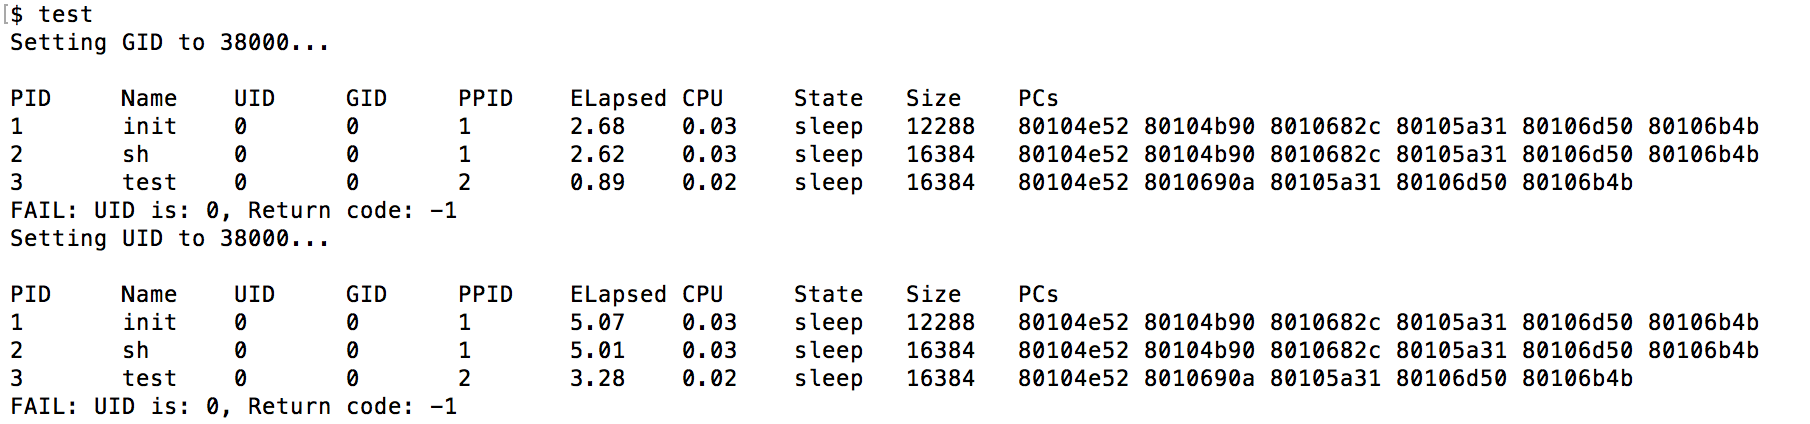
\includegraphics[width=0.8\linewidth]{invalid-setuid.png}
\caption[invalid setuid() and setgid()]{invalid setuid() and setgid()}
\label{fig:datetest}
\end{figure}	
	Because {\tt setgid()} and {\tt setuid()} were called with 38000, and ctrl-p shows the original GID/UID (unchanged) for test immediately after, and each call returned an
	error code of -1 this test \textbf{PASSES}.

\newpage	

\subsection*{getuid(), getgid() and getppid()}
	To test that {\tt getuid()}, {\tt getgid()}, {\tt getppid()} are working correctly each system call will be invoked in a function \emph{within} the {\tt test} user command. The result
	from each call, the IDs, will be printed to standard-out, and compared against the output from ctrl-p. We expect the printed UID, GID, and PPID printed from {\tt test} to match the 
	the information of the {\tt test} process in ctrl-p's output ({\tt test} is the process that these system calls are evoked from). We also expect that the PPID of {\tt test} will match the PID of 
	the shell process; because {\tt test} is forked from {\tt sh} (the shell process) and thus, {\tt sh} is its parent.

\begin{figure}[h!]
\centering
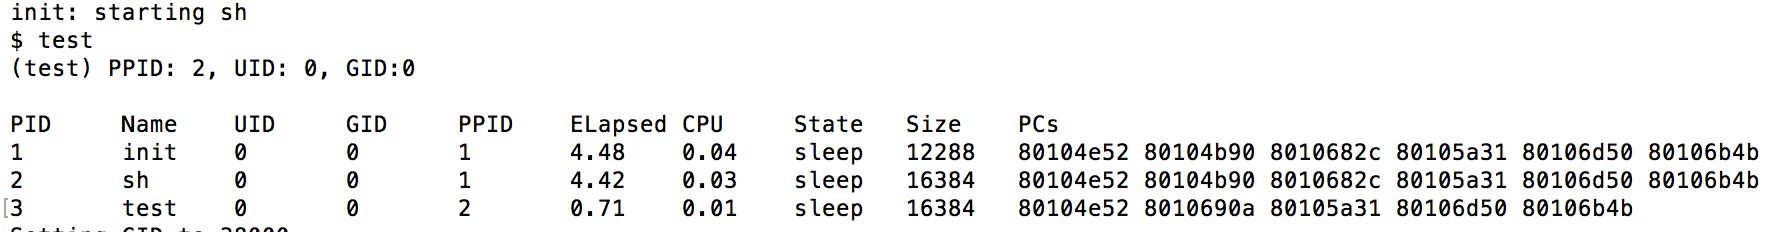
\includegraphics[width=0.8\linewidth]{test-all-get.png}
\caption[invalid setuid() and setgid()]{invalid setuid() and setgid()}
\label{fig:datetest}
\end{figure}

	In the figure above we can see that the output line of {\tt test} marked with "(test)" has a UID of 0, GID of 0, and PPID of 2. This matches the {\tt test} process information
	printed in ctrl-p's output immediately after. We also see that the PID of {\tt sh} is 2, which matches the PPID of {\tt test}. Because the {\tt ..get()} system call return values 
	match the process information output in ctrl-p and because the PPID of {\tt test} matched the PID of {\tt sh}, this test \textbf{PASSES}.


\newpage 

\subsection*{Built in shell commands for UID and GID}
	Next we will test whether the built in shell commands {\tt \_get uid}, {\tt \_get gid}, {\tt \_set uid int}, and {\tt \_set gid int} work correctly. To enable these commands for the shell
	we first must turn off the {\tt DUSE\_BUILTINS} flag in the Makefile (line 74). Next, since these system calls are invoked from the shell process, we will perform the following tests:

\subsection*{Built in shell commands for UID}	
	\begin{itemize}
			\item 1) ctrl-p to see the shell's starting UID
				
			\item 2) Call {\tt \_get uid} to verify this built in is working correctly
			
			\item 3) Call {\tt \_set uid} with a value $56$
			
			\item 4) Call {\tt \_get uid} to see the \emph{now current} UID value
			
			\item 5) Verify that the UID for {\tt sh} did change by pressing ctrl-p

	\end{itemize}
	
	When performing this test we expect to see: that the first call to {\tt \_get uid} matches the UID of {\tt sh} in ctrl-p's output; a return value of 0 for {\tt \_set uid} $56$; and a 
	subsequent {\tt \_get uid} return value of $56$ to match the second output of ctrl-p.

\begin{figure}[h!]
\centering
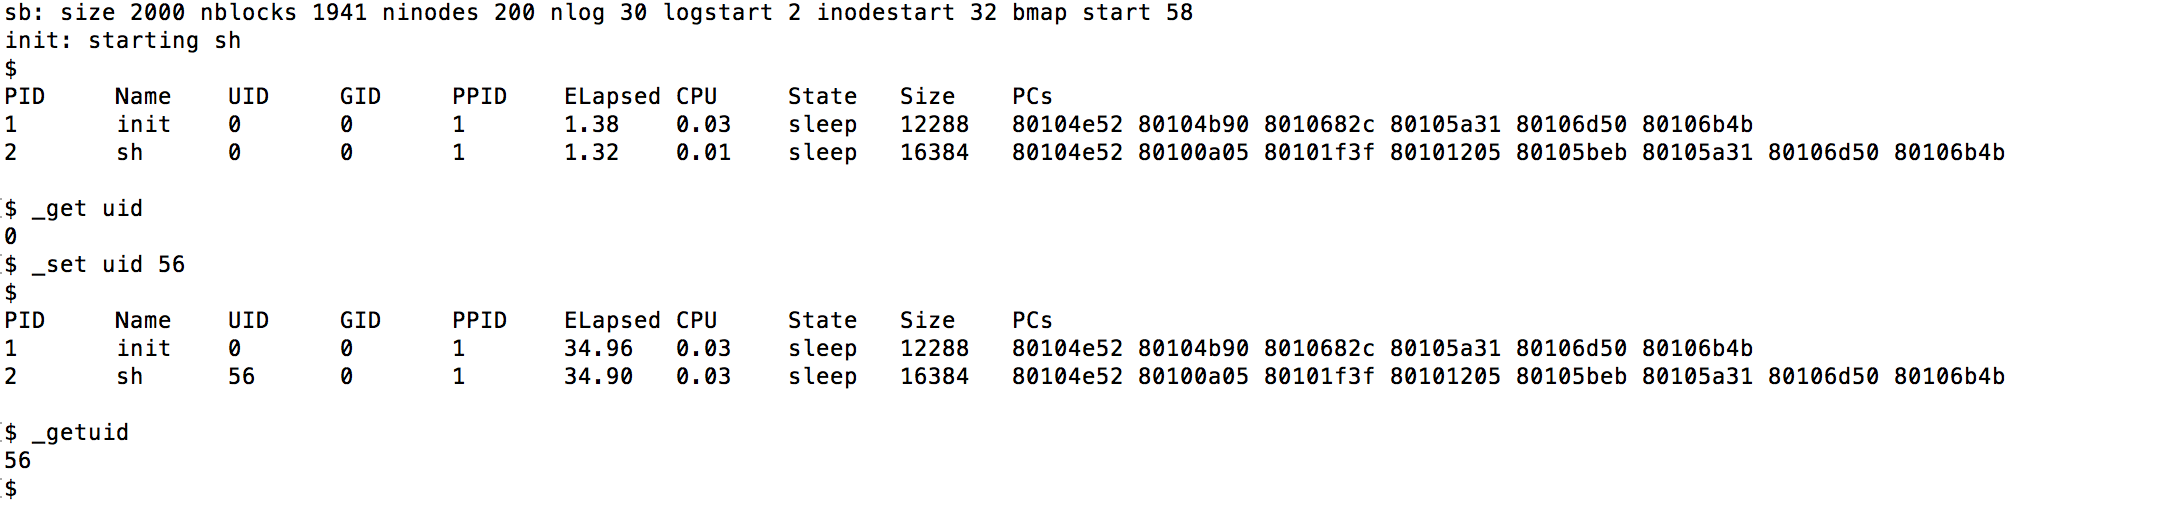
\includegraphics[width=0.8\linewidth]{shell-uid.png}
\caption[get/setuid (sh)]{get/setuid (sh)}
\label{fig:get/setuid}
\end{figure}

	Because the output of the test matches our expected output, a matching UID to ctrl-p's information, and a subsequent change to the new value where {\tt \_get uid} and 
	ctrl-p match again, this subtest \textbf{PASSES}.


\subsection*{Built in shell commands for GID}	
	\begin{itemize}
			\item 1) ctrl-p to see the shell's starting GID
				
			\item 2) Call {\tt \_get gid} to verify this built in is working correctly
			
			\item 3) Call {\tt \_set gid} with a value $71$
			
			\item 4) Call {\tt \_get gid} to see the \emph{now current} GID value
			
			\item 5) Verify that the GID for {\tt sh} did change by pressing ctrl-p

	\end{itemize}
	
	When performing this test we expect to see: that the first call to {\tt \_get uid} matches the GID of {\tt sh} in ctrl-p's output $1^st$ output;  and a 
	subsequent {\tt \_get uid} return value of $71$ to match the second output of ctrl-p (after having set the GID to 71).


\begin{figure}[h!]
\centering
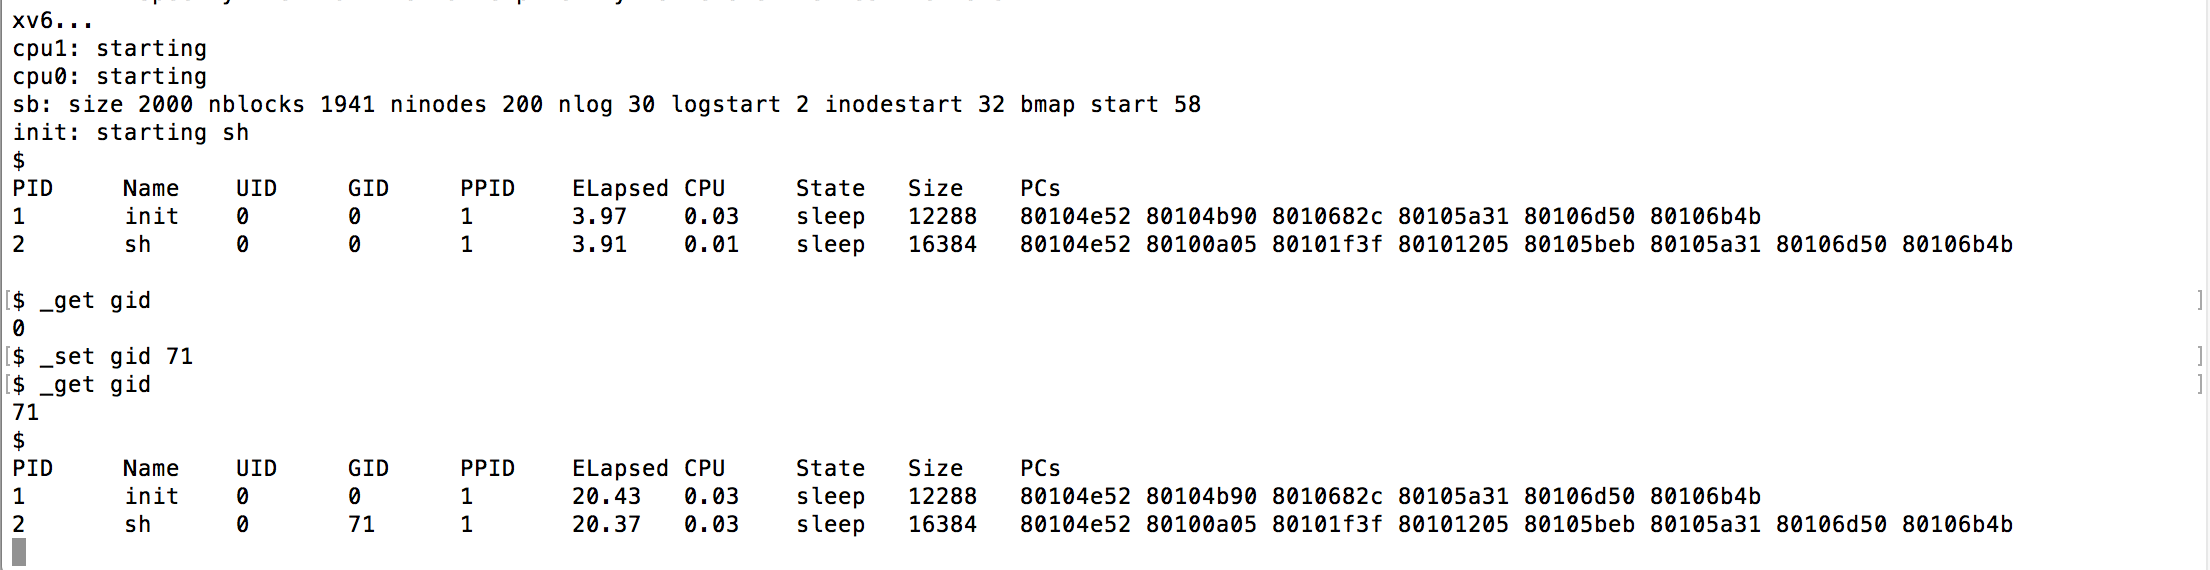
\includegraphics[width=0.7\linewidth]{shell-gid.png}
\caption[get/setgid (sh)]{get/setgid (sh)}
\label{fig:get/setgid (sh)}
\end{figure}

	Because the output of the test matches our expected output, a matching GID to ctrl-p's information, and a subsequent change to the new value where {\tt \_get gid} and 
	ctrl-p match again, this subtest \textbf{PASSES}.


	Because both subtests \textbf{PASS}, this test \textbf{PASSES}.
	
	
	
\subsection*{Fork() and ID inheritance}	

	To test that the GID and UID are properly inherited from the parent process we will write a program that sets its UID and GID, prints it, then forks and has the child process print 
	\emph{its} UID and GID. We expect that the UID and GID will match the parent process's UID and GID. Although test getuid(), getgid() and getppid() already demonstrated that 
	getppid() behaves as expected, we will again have the parent process prints its PID, and the child its PPID; we expect these to match.


\begin{figure}[h!]
\centering
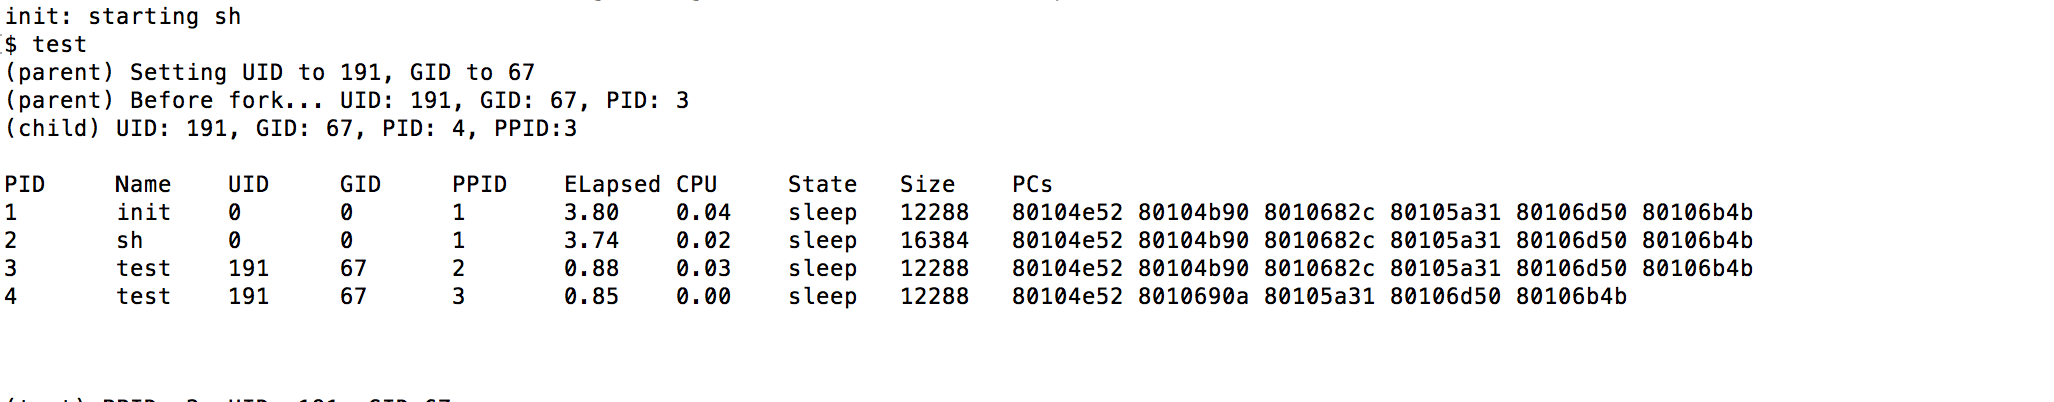
\includegraphics[width=.9\linewidth]{fork-test.png}
\caption[fork test]{fork test}
\label{fig:fork test}
\end{figure}

	From the output, it is clear that the parent was successful in setting its UID to 191 and GID to 67 (fork\_test() in test.c also checks the return code of each system call). In the 
	subsequent line we also see that the child has the same UID of 191 and GID of 67; this assertion by the child is verified by using ctrl-p's output to examine that both the parent
	(PID 3) and child (PID 4) have these values set. Additionally, we see that the child's PPID is 3, which is in fact its parent. Thus, this test \textbf{PASSES}.
	

\subsection*{PS command and getprocs() system call}	
	To test that the {\tt ps} user command, and consequently it's {\tt getprocs()} system call dependency,
	 is working correctly we will recompile the program with maximum values of 1, 16, 64, and 72, and have {\tt ps} print its current maximum
	value. Each time we will run {\tt ps} then immediately use ctrl-p to dump all currently active processes. 
	
	We expect that {\tt ps} will print either it's compiled maximum number of processes (1, 16, 64, or 72), \emph{or} the total number of processes active, which ever is least; for example
	if there are 12 active processes but {\tt ps} has a maximum value of 64, we expect to see 13 processes displayed (12 plus {\tt ps}), while on the other hand if there are 100 processes active and {\tt ps}
	has a maximum value of 4, we expect to see 4 processes displayed. Further, for the output of {\tt ps} we expect the PID, UID, GID, and PPID fields to match the output in ctrl-p, with the 
	Elapsed Time field being larger in ctrl-p. PCs will not be printed in {\tt ps} and we cannot make any assertions about the CPU field other than if it changes, it must increase. We cannot
	guarantee that the Size field will not change either.
		
	We also expect that since {\tt ps} gets active processes while it is running, that it ({\tt ps}) itself will be displayed in the table as long as
	 the maximum value it is compiled is larger than than the total number of other active processes. For example with a maximum value of 1 cannot guarantee that {\tt ps} will be the
	 process displayed since there will be more than one process active at that time (i.e. {\tt sh, init}). The results of these runs and the PASS/FAIL status are broken into 
	 into the following subtests.

\subsection*{PS command with a maximum of 1}

\begin{figure}[h!]
\centering
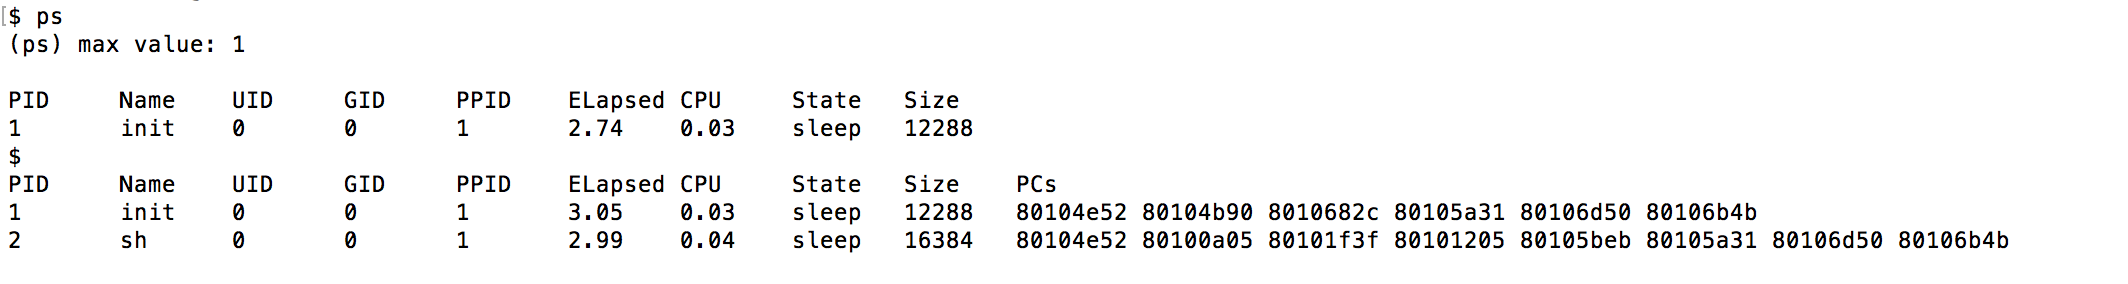
\includegraphics[width=.9\linewidth]{ps-1.png}
\caption[ps-1]{ps-1t}
\label{fig:ps-1}
\end{figure}

	The PID, UID, GID, and PPID fields printed by {\tt ps} match the respective output in ctrl-p; the elapsed time increases between {\tt ps} and ctrl-p; the 
	CPU time does not decrease; and the number of processes printed is one, so the results match our expectations for a maximum value of one. Thus, this subtest \textbf{PASSES}.

\subsection*{PS command with a maximum of 16}

\begin{figure}[h!]
\centering
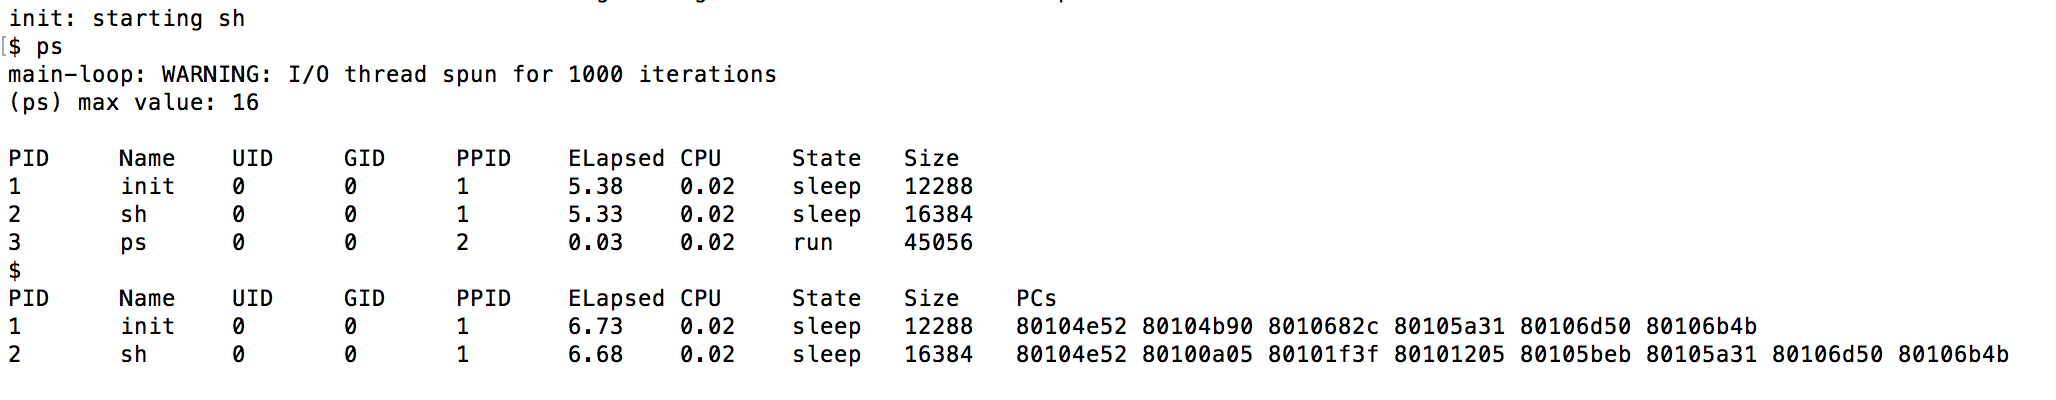
\includegraphics[width=.9\linewidth]{ps-16.png}
\caption[ps-16t]{fps-16}
\label{fig:ps-16}
\end{figure}

The PID, UID, GID, and PPID fields printed by {\tt ps} match the respective output in ctrl-p; the elapsed time increases between {\tt ps} and ctrl-p; the 
	CPU time does not decrease; the number of processes printed by {\tt ps} is 3 which is the total number active processes \emph{including} {\tt ps} (i.e. 
	 one greater than ctrl-p),
	 so the results match our expectations for a maximum value value that is larger than the number of current processes. Thus, this subtest \textbf{PASSES}.

\subsection*{PS command with a maximum of 64}

\begin{figure}[h!]
\centering
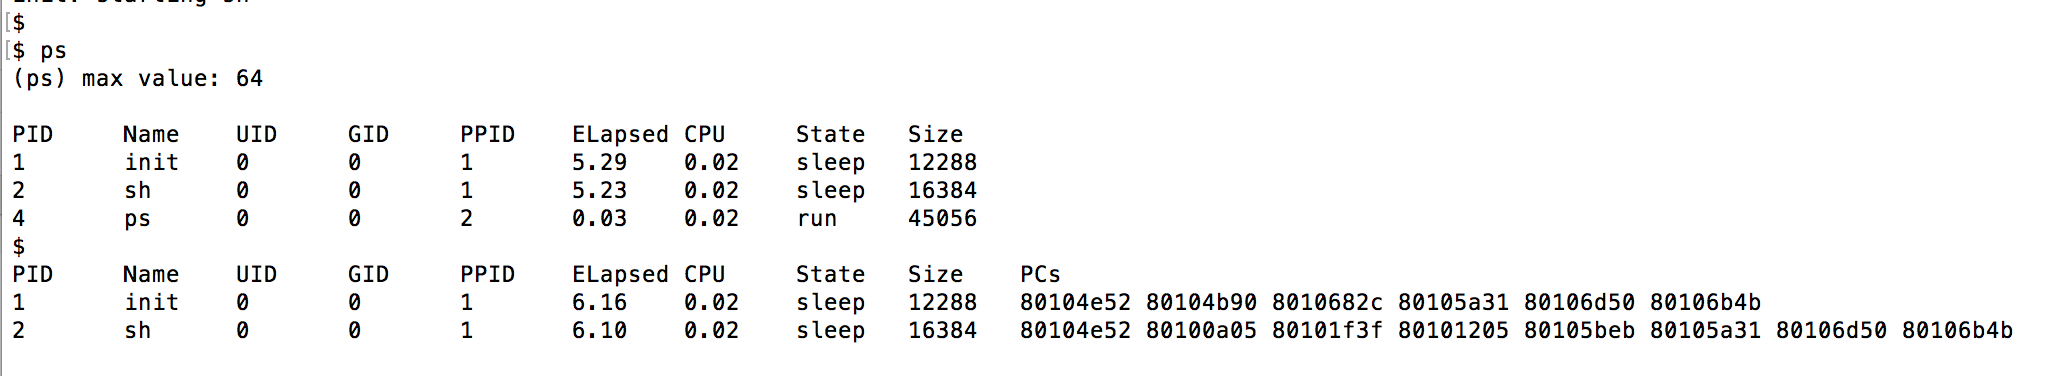
\includegraphics[width=.9\linewidth]{ps-64.png}
\caption[ps-64t]{ps-64}
\label{fig:fps-64}
\end{figure}

The PID, UID, GID, and PPID fields printed by {\tt ps} match the respective output in ctrl-p; the elapsed time increases between {\tt ps} and ctrl-p; the 
	CPU time does not decrease; the number of processes printed by {\tt ps} is 3 which is the total number active processes \emph{including} {\tt ps} (i.e. 
	 one greater than ctrl-p),
	 so the results match our expectations for a maximum value value that is larger than the number of current processes. Thus, this subtest \textbf{PASSES}.

\newpage

\subsection*{PS command with a maximum of 72}

\begin{figure}[h!]
\centering
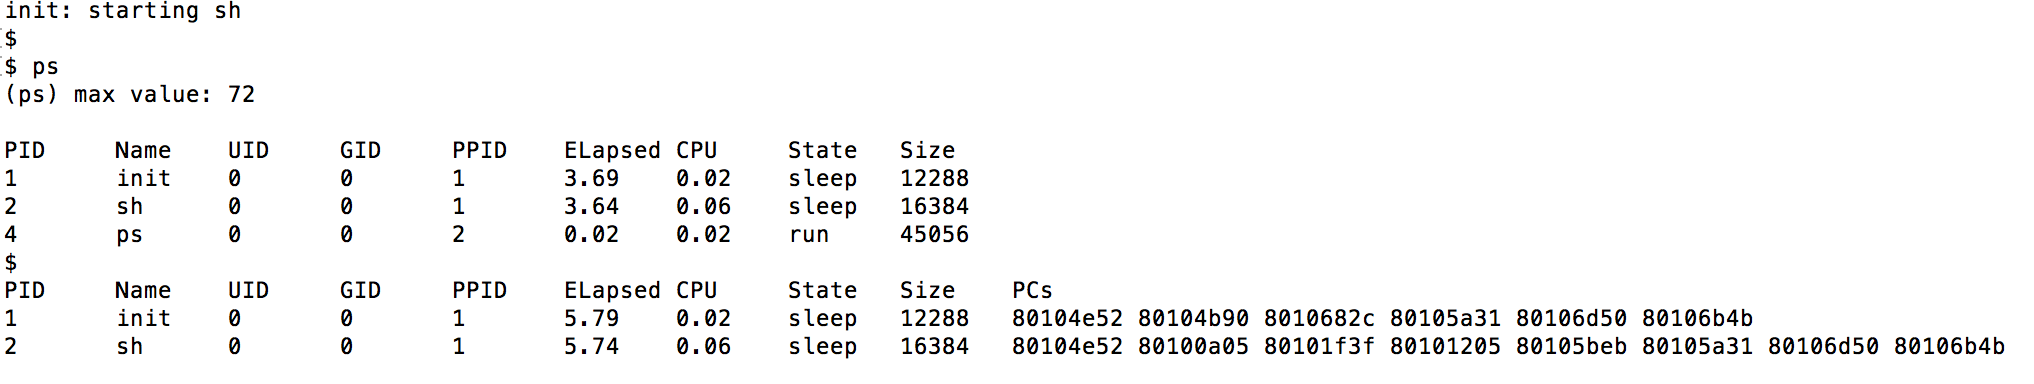
\includegraphics[width=.9\linewidth]{ps-72.png}
\caption[ps-72t]{ps-72}
\label{fig:ps-72}
\end{figure}
	  
	The PID, UID, GID, and PPID fields printed by {\tt ps} match the respective output in ctrl-p; the elapsed time increases between {\tt ps} and ctrl-p; the 
	CPU time does not decrease; the number of processes printed by {\tt ps} is 3 which is the total number active processes \emph{including} {\tt ps} (i.e. 
	 one greater than ctrl-p),
	 so the results match our expectations for a maximum value value that is larger than the number of current processes. Thus, this subtest \textbf{PASSES}.

Because all subtests passed, this test \textbf{PASSES},

\subsection*{CPU Time}

	To test that the CPU time is displaying properly, we will press ctrl-p to identify the CPU time for the shell process {\tt sh}, then we will hit the return key repeatedly 
	forcing {\tt sh} to process null commands and thus increase it's CPU usage. Then we will hit ctrl-p to see its CPU time again. We expect that since the the {\tt sh}
	processed multiple null commands, and it must do so using the CPU, that it's CPU time will have increased. More so, we expect this increase to be approximate 
	to the \emph{difference} in Elapsed Time field values of ctrl-p. The result is as follows:

\begin{figure}[h!]
\centering
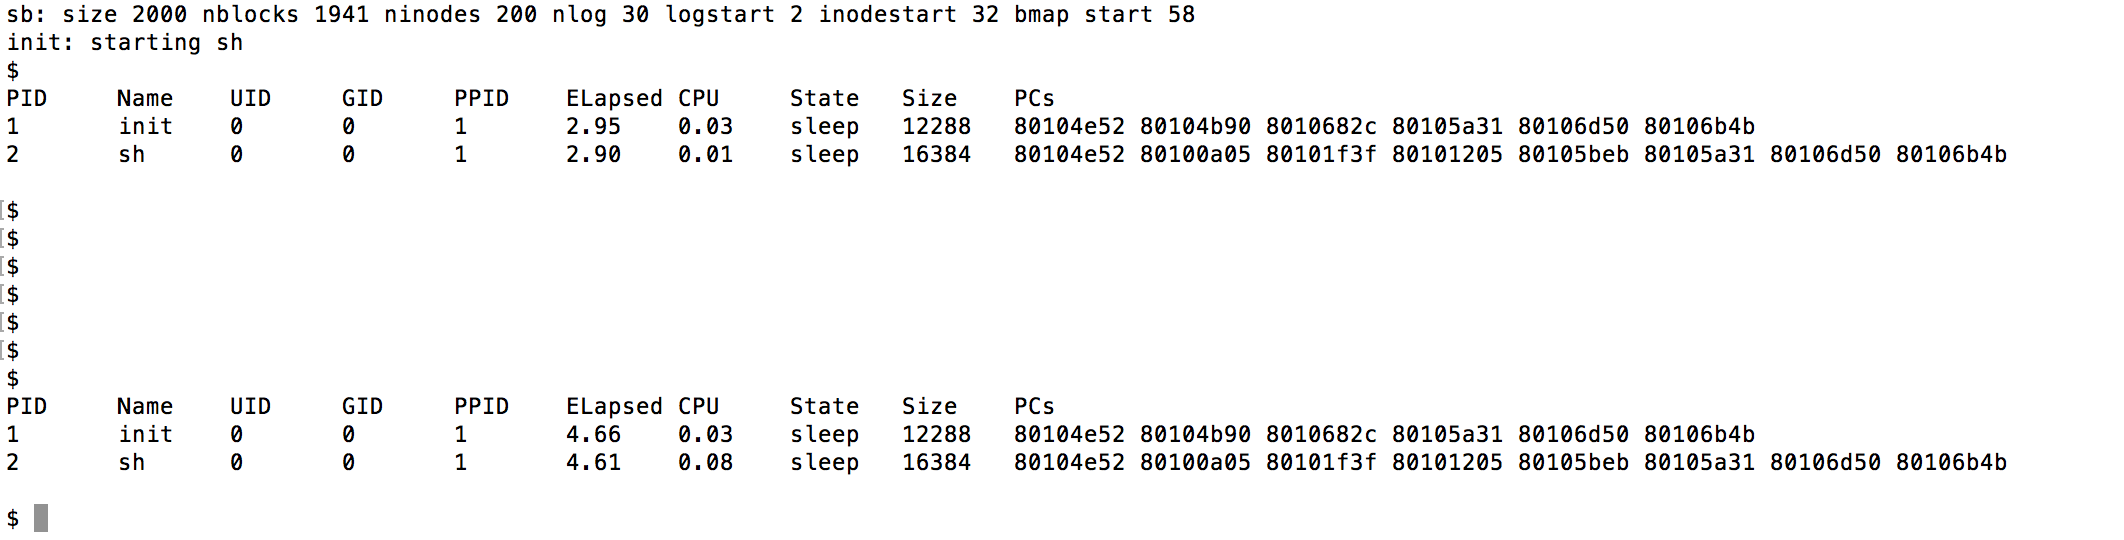
\includegraphics[width=.9\linewidth]{cpu-time.png}
\caption[cpu time]{CPU time}
\label{fig:cpu}
\end{figure}
	
	As the results illustrate, the CPU time of {\tt sh} did increase by 0.07 seconds between the initial and final ctrl-p outputs. Thus this test \textbf{PASSES}.
	
\subsection*{time command}
	To test the {\tt time} user command, we will establish subtests for executing; {\tt time}, {\tt time ls}, {\tt time echo abc}, {\tt time time echo time}, and 
	{\tt time badcommand!}. Since expectations differ for each execution subtests will be established.

\subsection*{time (null)}
	For the execution of {\tt time} we expect the {\tt null} command will be timed, and should complete in \emph{approximately} 0.00 seconds (set up of execution takes
	non-zero time), so we expect {\tt time} to display
	that the {\tt null} command executed in such a time.
	
	\begin{figure}[h!]
\centering
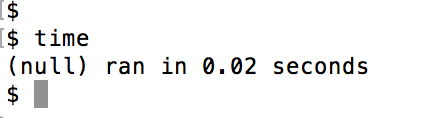
\includegraphics[width=.6\linewidth]{time-null.png}
\caption[timenull]{time null}
\label{fig:timenull}
\end{figure}
	
	Because {\tt time} printed the command (null) and stated its execution was 0.02 which is approximately 0.00, this subtest \textbf{PASSES}.
	
\subsection*{time ls}
	For the execution of {\tt time ls} we expect that the execution of {\tt ls} will take non-zero time, within a reasonable range of under 1 second. We also expect that we will
	see the output of {\tt ls} before we see the output of {\tt time}.
	
	\begin{figure}[h!]
\centering
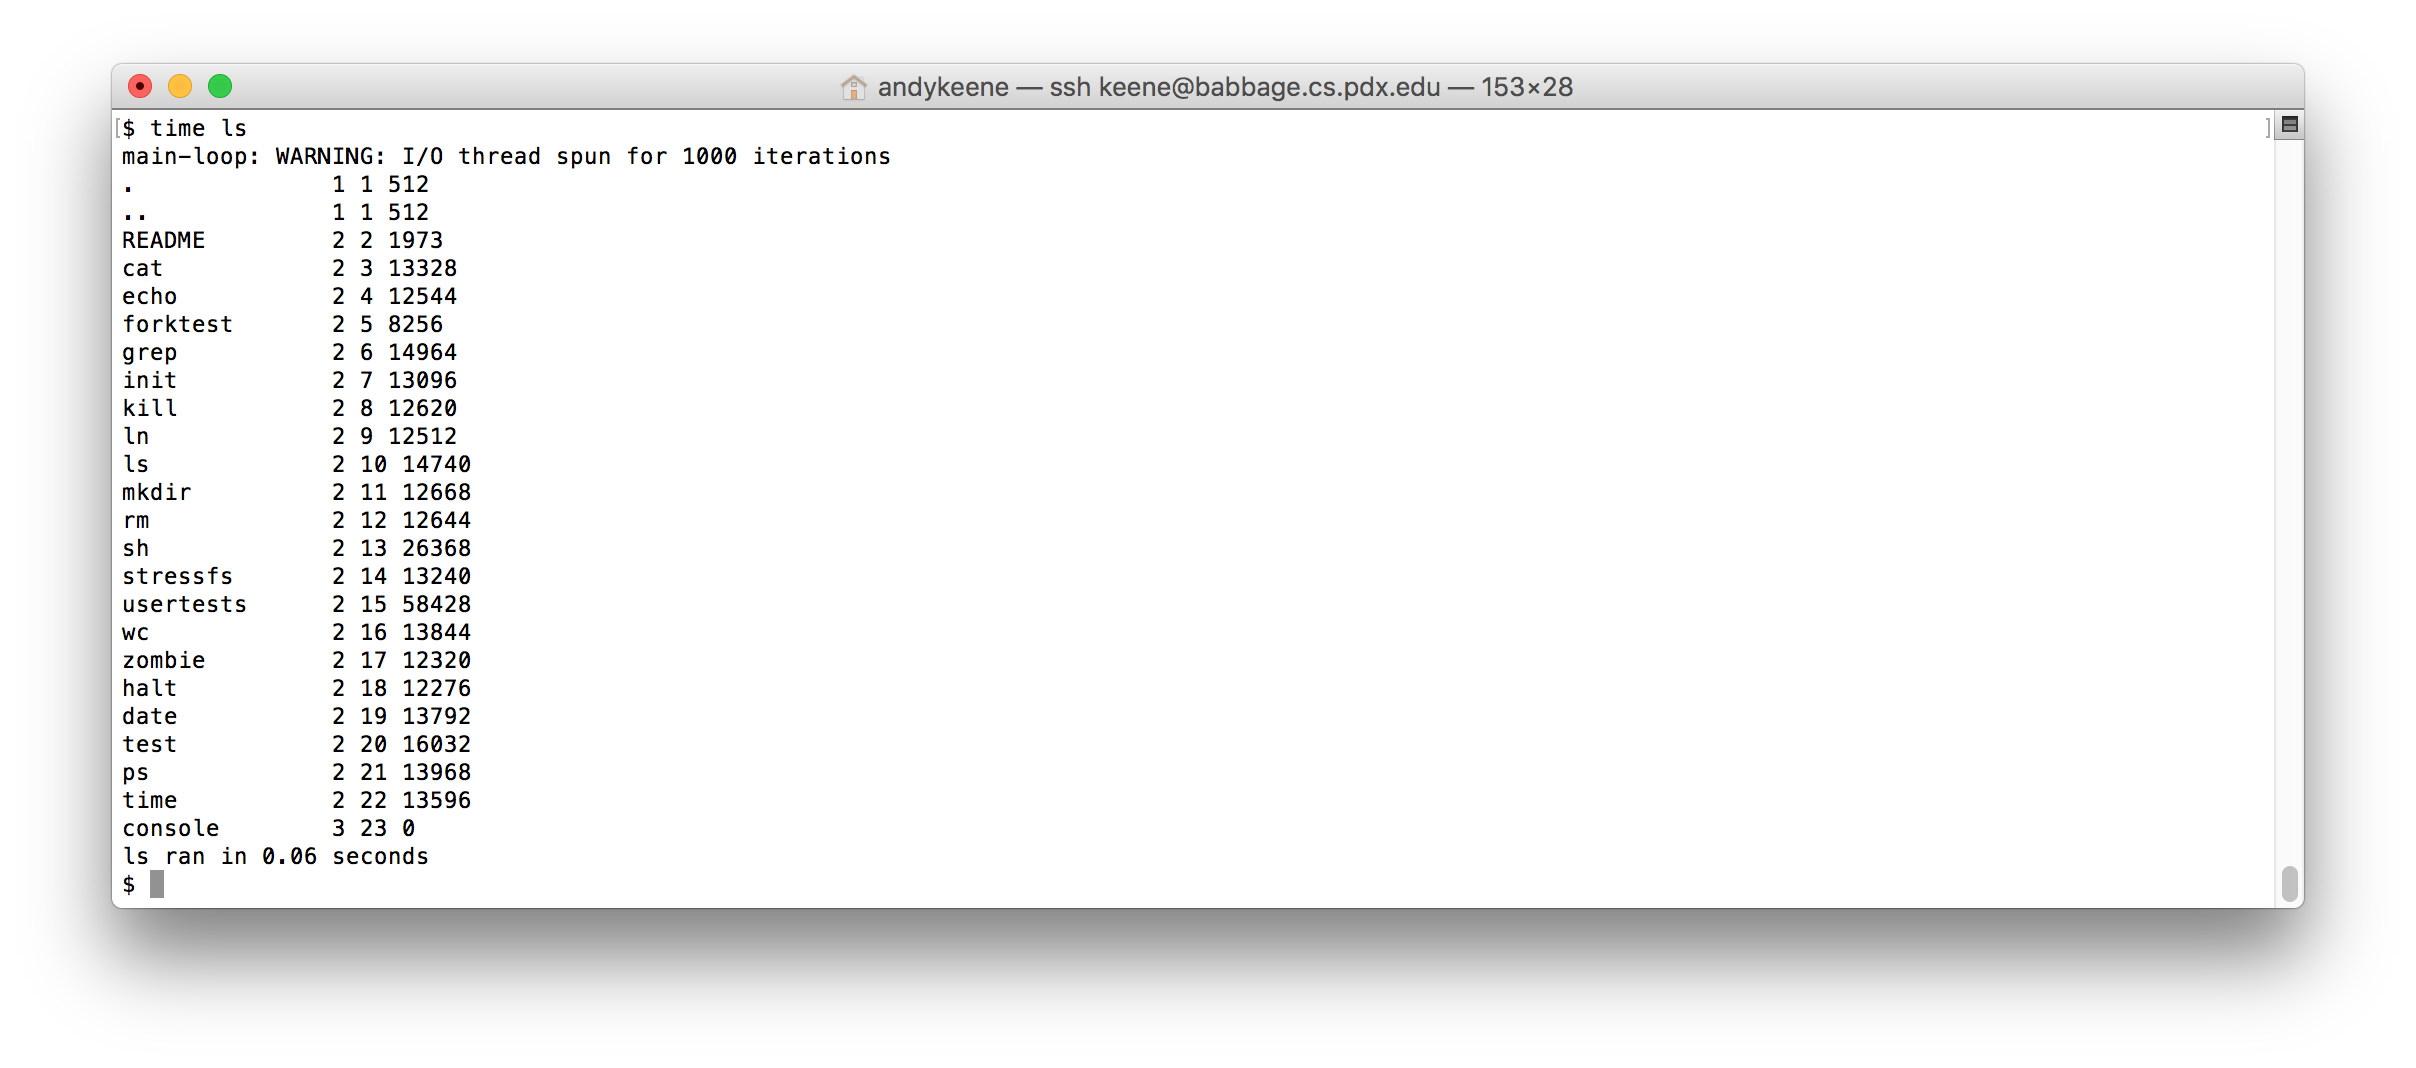
\includegraphics[width=.9\linewidth]{time-ls.png}
\caption[timels]{time ls}
\label{fig:timels}
\end{figure}
	
	Because the output of {\tt ls} appears first, followed by {\tt time}s output that ls ran in 0.6 seconds (within reason of 1 second) this subtest \textbf{PASSES}.
	
\subsection*{time echo abc}
	For the execution of {\tt time echo abc} we expect that the execution of {\tt echo abc} will take non-zero time, within reason. We also expect that we will
	see the output of {\tt echo abc} before we see the output of {\tt time} since {\tt abc} is the argument to {\tt echo}.
	
\begin{figure}[h!]
\centering
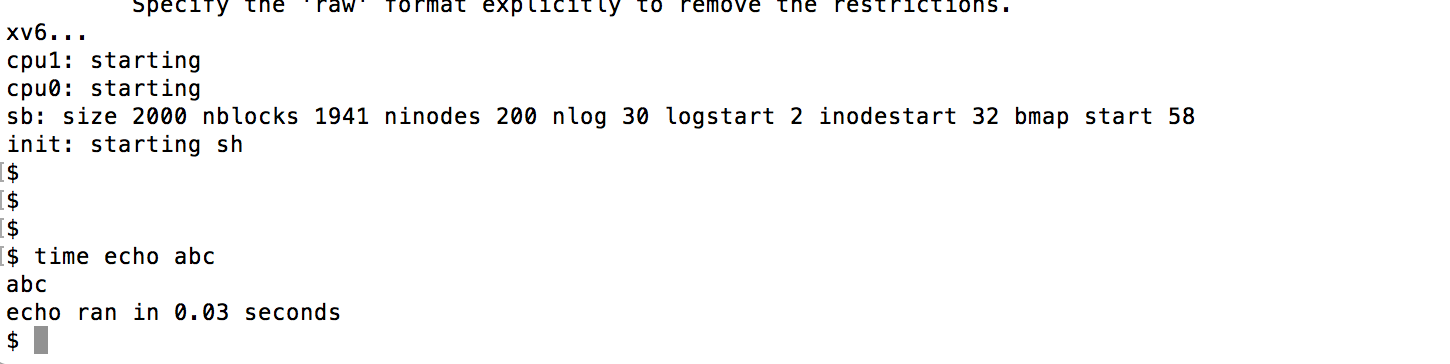
\includegraphics[width=.9\linewidth]{time-echo.png}
\caption[timels]{time echo abc}
\label{fig:timels}
\end{figure}
	
	Because the output of {\tt echo abc} appears first (where {\tt abc} was the argument for {\tt echo}, followed by {\tt time}s output that echo ran in 0.03 seconds (within reason) this subtest \textbf{PASSES}.
	
\newpage

\subsection*{time time echo abc}
	For the execution of {\tt time time echo abc} we expect that the execution of {\tt echo abc} will print to standard-out. Following {\tt echo}s output we expect to see, like before,
	that {\tt echo} ran in non-zero time (approximately 0.03 seconds as established) from the \emph{second} {\tt time} command, finally followed by a {\tt time ran in ... } output from the
	first {\tt time} command timing the second {\tt time}, where this time must be greater than the execution time of {\tt echo abc}.
	
\begin{figure}[h!]
\centering
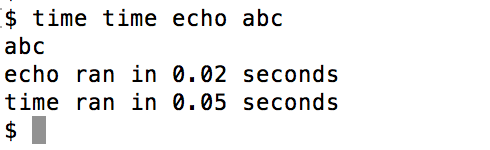
\includegraphics[width=.7\linewidth]{time-time.png}
\caption[timetimels]{time time echo abc}
\label{fig:timetimeecho}
\end{figure}
	
	Because the output of {\tt echo abc} appears first, followed by a reasonable time of {\tt echo} (0.02 seconds) by the second {\tt time} command and because we see an 
	output of {\tt time ran in 0.05 seconds} which is greater than the execution time of {\tt echo} alone, this subtest \textbf{PASSES} and ensures the generality of the {\tt time} command.

\newpage

\subsection*{time badcommand}
	To verify {\tt time} will respond to a failure to execute a command and time it, we will test the execution of {\tt time badcommand}. {\tt time} was implemented to throw an error on failure 
	to execute a command, but \emph{not} to exit; because we may still want to see timings from the commands that before the failure. 
	As a result of this implementation choice, we expect to see that when given a bad command (i.e. {\tt badcommand}) that an error will be displayed that the command did not execute, but 
	{\tt time} will still report a time for the execution (the attempted execution) of the bad command before exiting normally. Also, due to our expectations that {\tt badcommand} will fail to
	execute, we expect an attempted run time zero seconds.
	
\begin{figure}[h!]
\centering
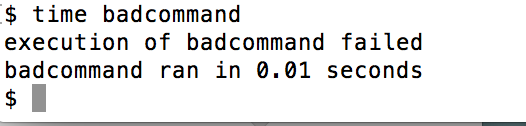
\includegraphics[width=.7\linewidth]{time-badcommand.png}
\caption[timebadcommand]{time-badcommand}
\label{fig:timebadcommand}
\end{figure}
	

	Because {\tt time badcommand} prompted the user that {\tt badcommand} failed, but still reported a time of 0.01 seconds (near zero seconds) for its attempted execution, this test behaves 
	according to the expectations
	set by its implementation. Thus, this test \textbf{PASSES}.
	
\end{document}




